\section{Theory}
To facilitate a better understanding of the heuristic methods presented in this protocol, key concepts must first be introduced.

\paragraph{Problem}
In the context of this protocol, a \textit{problem} represents a project that is made up of activities.
Each activity takes a certain amount of time to complete and a set amount of resources at each point in time.
To complete the project, all activities must be finished while adhering to their dependencies and the resources available for the project at each point in time.
The challenging aspect of the problem is to complete the project in the shortest time possible while keeping to the dependencies, and not exceeding the resources available. The activities and their relationships within a project can be represented using an event-oriented directed graph, called the \textit{CPM network}.

In a CPM network, the nodes represent milestones that mark the start or completion of activities, while the directed, weighted edges represent the activities and their duration.
For this project, it is assumed that there is only one start node initiating the project and one end node that represents the completion of the project.
An example of such a graph is presented in Figure~\ref{Figure:theory->problem->cpm-network-example}.

\begin{figure}[ht!]
	\centering
	\begin{tikzpicture}[
		mynode/.style={
			circle,
			draw=black,
			fill=gray,
			fill opacity = 0.3,
			text opacity=1,
			inner sep=0pt,
			minimum size=20pt,
			font=\small},
		myarrow/.style={-Stealth},
		node distance=0.6cm and 1.2cm
		]
		\node[mynode] (n1) {1};
		\node[mynode,above right=of n1] (n2) {2};
		\node[mynode,below=of n2] (n3) {3};
		\node[mynode,below=of n3] (n4) {4};
		\node[mynode,right=of n3] (n5) {5};
		\node[mynode,right=of n5] (n6) {6};
		
		\foreach \i/\j/\txt/\p in {% start node/end node/text/position
			n1/n2/4/above,
			n1/n3/3/above,
			n1/n4/5/above,
			n2/n5/3/above,
			n3/n5/2/above,
			n4/n6/4/below,
			n5/n6/3/above}
			\draw [myarrow] (\i) -- node[sloped,font=\small,\p] {\txt} (\j);
			
	\end{tikzpicture}
	\caption{Visualization of a project comprising activities as a CPM network.
		Each node represents a milestone that either marks the start or the completion of activities.
		The number inside each node is the ID of the milestone represented by the node.
		Each weighted edge represents an activity and its duration.
		The ID of an activity is dependent on the node it starts from and the node it ends in, i.e. $i$-$j$, where $i$ is the ID of the start node and $j$ is the ID of the end node.
		For example, the ID of the activity starting in node 1 and ending in node 2 is 1-2 and its duration is 4.
	}
	\label{Figure:theory->problem->cpm-network-example}
\end{figure}

For clarity, the term \textit{dependency of activities} means that an activity cannot be started before all of its predecessors have been completed. For example, in Figure~\ref{Figure:theory->problem->cpm-network-example}, activity 5-6 can only be started once activities 2-5 and 3-5 have been completed.

The graph presented in Figure~\ref{Figure:theory->problem->cpm-network-example} is referred to as a CPM network due to its widespread use during the analysis of projects using the Critical Path Method (CPM) \cite{Kelley1959}.

\paragraph{Critical Path Method (CPM)}
The Critical Path Method is an algorithm used for scheduling activities of a project.
It is used to determine the earliest possible end of the project while only adhering to the dependencies of activities and their durations, i.e., not their resources.
Given its dependencies and duration ($t_{i, j}$), for each activity, the algorithm of CPM determines the following: 

\begin{tight_itemize}
	\item Earliest Start (ES) - Earliest possible time the activity can \textit{start} considering its dependencies.
	\item Earliest End (EE) - Earliest possible time the activity can \textit{end} considering its dependencies.
	\item Latest Start (LS) - Latest permissible time the activity can \textit{start} considering its dependencies.
	\item Latest End (LE) - Latest permissible time the activity can \textit{end} considering its dependencies.
	\item Time Reserves (TR) - Number of time units that the activity can be delayed before the end of the project must be delayed.
		It is equal to the difference between LE and EE (or LS and ES).
\end{tight_itemize}

If the time reserves for an activity are equal to zero, then delaying the activity means delaying the project.
Activities with zero time reserves are referred to as \textit{critical activities} and they make up the so-called \textit{critical path}.
The critical path is a sequence of dependent activities between the start and end nodes that dictates when the project can be completed earliest.

For example, the output of CPM for the project shown in Figure~\ref{Figure:theory->problem->cpm-network-example} is presented in Table~\ref{Table:theory->cpm->exmaple->data}.

\begin{table}[ht]
	\centering
	\begin{tabular}{|c|c|c|c|c|c|c|}
		\hline
		$i$-$j$ & $t_{i, j}$ & ES$_{i, j}$ & EE$_{i, j}$ & LS$_{i, j}$ & LE$_{i, j}$ & TR$_{i, j}$ \\ \hline
		  1-2   &     4      &      0      &      4      &      0      &      4      &      0      \\
		  1-3   &     3      &      0      &      3      &      2      &      5      &      2      \\
		  1-4   &     5      &      0      &      5      &      1      &      6      &      1      \\
		  2-5   &     3      &      4      &      7      &      4      &      7      &      0      \\
		  3-5   &     2      &      3      &      5      &      5      &      7      &      2      \\
		  4-6   &     4      &      5      &      9      &      6      &     10      &      1      \\
		  5-6   &     3      &      7      &     10      &      7      &     10      &      0      \\ \hline
	\end{tabular}
	\caption{Output of CPM for the project presented in Figure~\ref{Figure:theory->problem->cpm-network-example}.
		The critical path is made up of activities 1-2, 2-5, and 5-6 since their TRs are equal to zero.
		The last activities, 4-6 and 5-6, are both completed at time unit 10, therefore, the entire project can be completed in 10 time units.
	}
	\label{Table:theory->cpm->exmaple->data}
\end{table}

The activity timeline produced by CPM can be visualized using a Gantt chart\footnote{Gantt chart Wikipedia URL: \url{https://en.wikipedia.org/wiki/Gantt_chart}}, as shown in Figure~\ref{Figure:theory->cpm->example->timeline}.

\afterpage{
\begin{figure}[ht!]
	\centering
	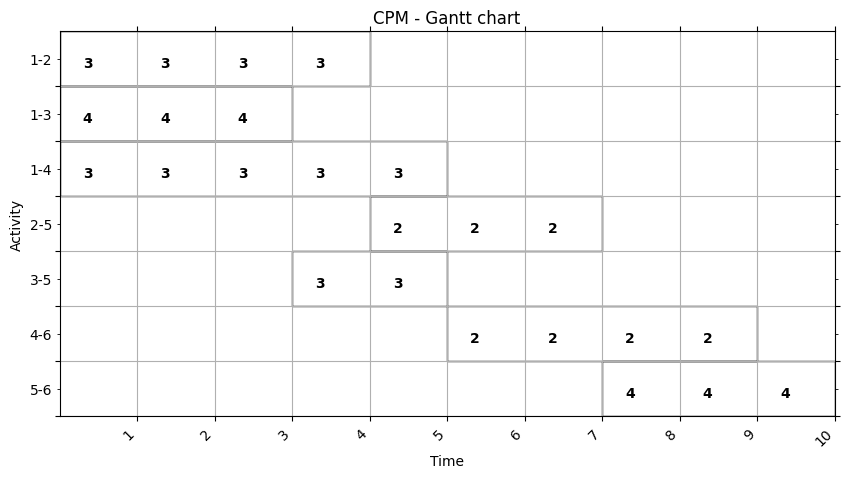
\includegraphics[width=\linewidth]{images/cpm_example_project.png}
	\caption{Timeline of the activities presented in Table~\ref{Table:theory->cpm->exmaple->data} as scheduled by CPM.
		The vertical axis represents the activity, while the horizontal axis displays the time units.
		The numbers in the squares represent the units of resources required by each activity at a point in time.
		Note that CPM does not take the resources into account, they are only displayed here for completeness.
		The image was generated using the Matplotlib Python package\protect\footnotemark[2].
	}
	\label{Figure:theory->cpm->example->timeline}
\end{figure}
\footnotetext[2]{Matplotlib webpage URL: \url{https://matplotlib.org/stable/index.html}}
}

The algorithm of CPM is omitted as the output of CPM is the input for the heuristic methods that schedule the activities of a project while adhering to the dependencies, the durations, and the resources.

\subsection{Heuristic Methods}
As mentioned earlier, CPM determines the earliest possible end of a project while taking into account only the dependencies of activities and their durations.
On the other hand, the heuristic methods analyzed in this protocol also take into account the resources required by each activity at a point in time.

The heuristic methods selected from from \citetitle{Fiala2008} \cite{Fiala2008} for this assessment project are the following:

\begin{tight_itemize}
	\item Serial Heuristic Method (SHM)
	\item Parallel Heuristic Method (PHM)
	\item Parallel Heuristic Method with Dynamic Priorities (PHMDP)
\end{tight_itemize}

All of the above-mentioned heuristic methods use the output of CPM as their input.
Additionally, the heuristic methods take in the $r_\mathrm{max}$ parameter which represents the maximum number of resources available at each point in time.



\subsection{Serial Heuristic Method (SHM)}
Using the output of CPM and the provided $r_\mathrm{max}$, the Serial Heuristic Method performs the following steps:

\begin{tight_enumerate}
	\item Arrange the activities into a sequence $\left(i_1, j_1\right),  \ldots, \left(i_m, j_m\right)$ so that $i_k < i_{k+1}, j_k < j_{k+1}$.
	\item Starting with the first activity, schedule each activity while adhering to the dependencies and the maximum resources available at a point in time ($r_\mathrm{max}$).
\end{tight_enumerate}

To demonstrate the process, the activity timeline for the example project scheduled using SHM with $r_\mathrm{max} = 6$ is shown in Figure~\ref{Figure:theory->shm->example->timeline}.

\begin{figure}[ht!]
	\centering
	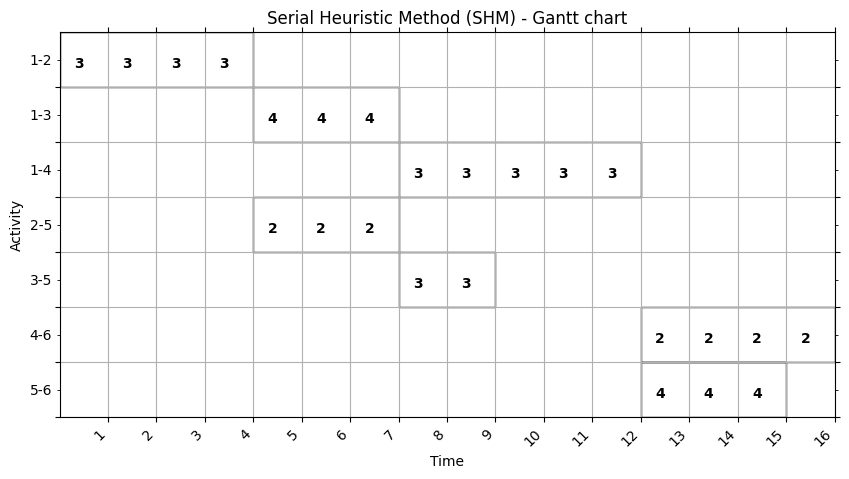
\includegraphics[width=\linewidth]{images/shm_example_project.png}
	\caption{Timeline of the activities presented in Table~\ref{Table:theory->cpm->exmaple->data} as scheduled by SHM.
		The vertical axis represents the activity, while the horizontal axis displays the time units.
		The numbers in the squares represent the units of resources required by each activity at a point in time.
	}
	\label{Figure:theory->shm->example->timeline}
\end{figure}

Specifically, the order of activities in the sequence is identical to the order of activities in column $\left(i, j\right)$ in Table~\ref{Table:theory->cpm->exmaple->data}.
SHM schedules activity 1-2 from time 0.
Then it tries to schedule activity 1-3, however, it can only do so from time 4 when activity 1-2 has finished as the resources required by both activities would exceed the resources available $3 + 4 = 7 > 6$.
According to SHM, the project can be completed in 16 time units while adhering to both dependencies and the available resources.

From Figure~\ref{Figure:theory->shm->example->timeline}, it can be seen that SHM is noticeably inefficient.
For example, from time 0, activities 1-2 and 1-4 can be scheduled while not exceeding the available resources.
However, since activity 1-3 is scheduled earlier, activity 1-4 cannot be scheduled until time unit 7.
This inefficiency is addressed by the \textit{Parallel Heuristic Method}.



\subsection{Parallel Heuristic Method (PHM)}
Unlike SHM, the Parallel Heuristic Method (PHM) provides each activity with a priority equal to its Time Reserves (TR) value.
Counterintuitively, the lower the priority value of an activity, the higher the priority of the activity.
This is due to TR representing the number of time units that an activity can be delayed for.
Thus, if $\mathrm{TR_{i ,j}} = 0$, then activity $i$-$j$ must be scheduled as soon as possible, otherwise the project may be delayed.

Using the output of CPM and the provided $r_\mathrm{max}$, PHM performs the following steps:

\begin{tight_enumerate}
	\item For every time unit:
	\begin{tight_enumerate}
		\item Create a set of activities whose predecessors are all completed.
		\item Arrange the activities in the set in ascending order according to their TR value.
		\item Starting with the activity with the lowest TR value, schedule as many activities from the time unit as possible while adhering to the resources available in every time unit.
	\end{tight_enumerate}
\end{tight_enumerate}

The activity timeline for the example project scheduled using PHM with $r_\mathrm{max} = 6$ is shown in Figure~\ref{Figure:theory->phm->example->timeline}.

\begin{figure}[ht!]
	\centering
	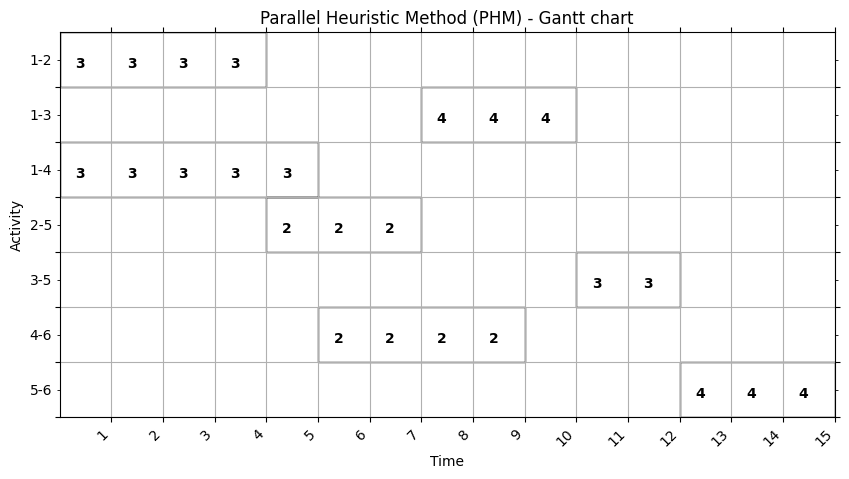
\includegraphics[width=\linewidth]{images/phm_example_project.png}
	\caption{Timeline of the activities presented in Table~\ref{Table:theory->cpm->exmaple->data} as scheduled by PHM.
		The vertical axis represents the activity, while the horizontal axis displays the time units.
		The numbers in the squares represent the units of resources required by each activity at a point in time.
	}
	\label{Figure:theory->phm->example->timeline}
\end{figure}

As can be seen from Figure~\ref{Figure:theory->phm->example->timeline}, unlike SHM, PHM scheduled activities 1-2 and 1-4 to run parallel.
The prioritization of activities allows PHM to determine that the project can be completed in 15 time units while adhering to both the dependencies and available resources.

However, PHM has a weakness: statically set priorities.
The priorities set by PHM do not change with the flow of time.
Therefore, the completion of non-critical activities can be delayed, thus causing suboptimal scheduling.
For example, since the TR value of activity 1-3 is 2, its scheduling is delayed until time 7.
Therefore, activities 3-5 and 5-6 are not even considered until time 10 which delays the entire project.
This flaw is addressed using the \textit{Parallel Heuristic Method with Dynamic Priorities}.



\subsection{Parallel Heuristic Method with Dynamic Priorities (PHMDP)}
The Parallel Heuristic Method with Dynamic Priorities (PHMDP) sets the priority value of each activity to $\mathrm{LS}_{i, j} - t$, where $t$ represents the time.
Furthermore, for every $t$, PHMDP updates the priorities, which eliminates the inadequacy of PHM.

Using the output of CPM and the provided $r_\mathrm{max}$, PHMDP performs the following steps:

\begin{tight_enumerate}
	\item For every time unit $t$:
	\begin{tight_enumerate}
		\item Create a set of activities whose predecessors are all completed.
		\item Update the priorities for the activities to $\mathrm{LS}_{i, j} - t$.
		\item Arrange the activities in the set in ascending order according to their priority value.
		\item Starting with the activity with the lowest priority value, schedule as many activities from the time unit as possible while adhering to the resources available in every time unit.
	\end{tight_enumerate}
\end{tight_enumerate}

The activity timeline for the example project scheduled using PHMDP with $r_\mathrm{max} = 6$ is shown in Figure~\ref{Figure:theory->phmdp->example->timeline}.

\begin{figure}[ht!]
	\centering
	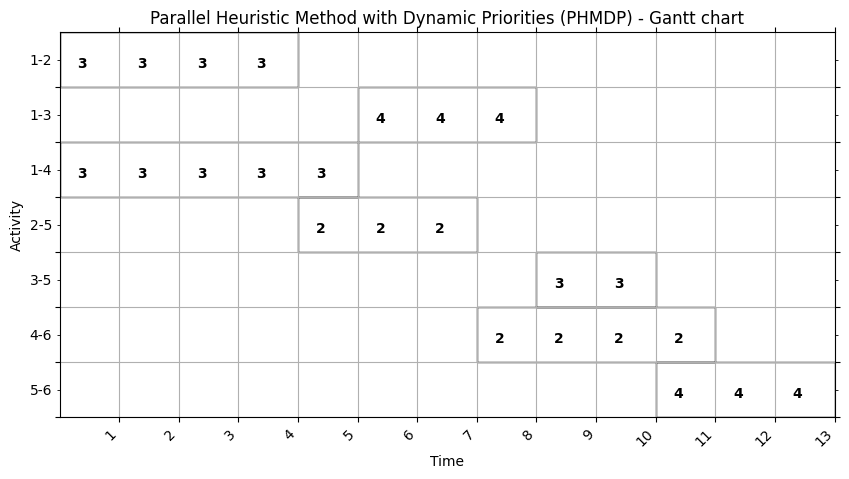
\includegraphics[width=\linewidth]{images/phmdp_example_project.png}
	\caption{Timeline of the activities presented in Table~\ref{Table:theory->cpm->exmaple->data} as scheduled by PHMDP.
		The vertical axis represents the activity, while the horizontal axis displays the time units.
		The numbers in the squares represent the units of resources required by each activity at a point in time.
	}
	\label{Figure:theory->phmdp->example->timeline}
\end{figure}

As shown in Figure~\ref{Figure:theory->phmdp->example->timeline} the dynamic priorities allow for activities to be scheduled more efficiently.
Ultimately, this results in PHMDP determining that the project can be completed in 13 time units while adhering to both the dependencies and available resources.

To examine the behavior of the methods further, they were implemented and compared on more examples.

